\chapter{Software Architecture Design}
\label{chap:software-architecture-design}

\section{Domain Model}
\label{section:domain-model}
The domain model of Spell Splash illustrates the core components and interactions of the game—players, 
vocabulary words, quizzes, challenges, and rewards. It demonstrates how gameplay supports vocabulary 
learning through engaging activities like battles and puzzles, connecting educational goals with interactive 
mechanics to make English learning more effective and enjoyable.
\begin{figure}[H]
    \centering
    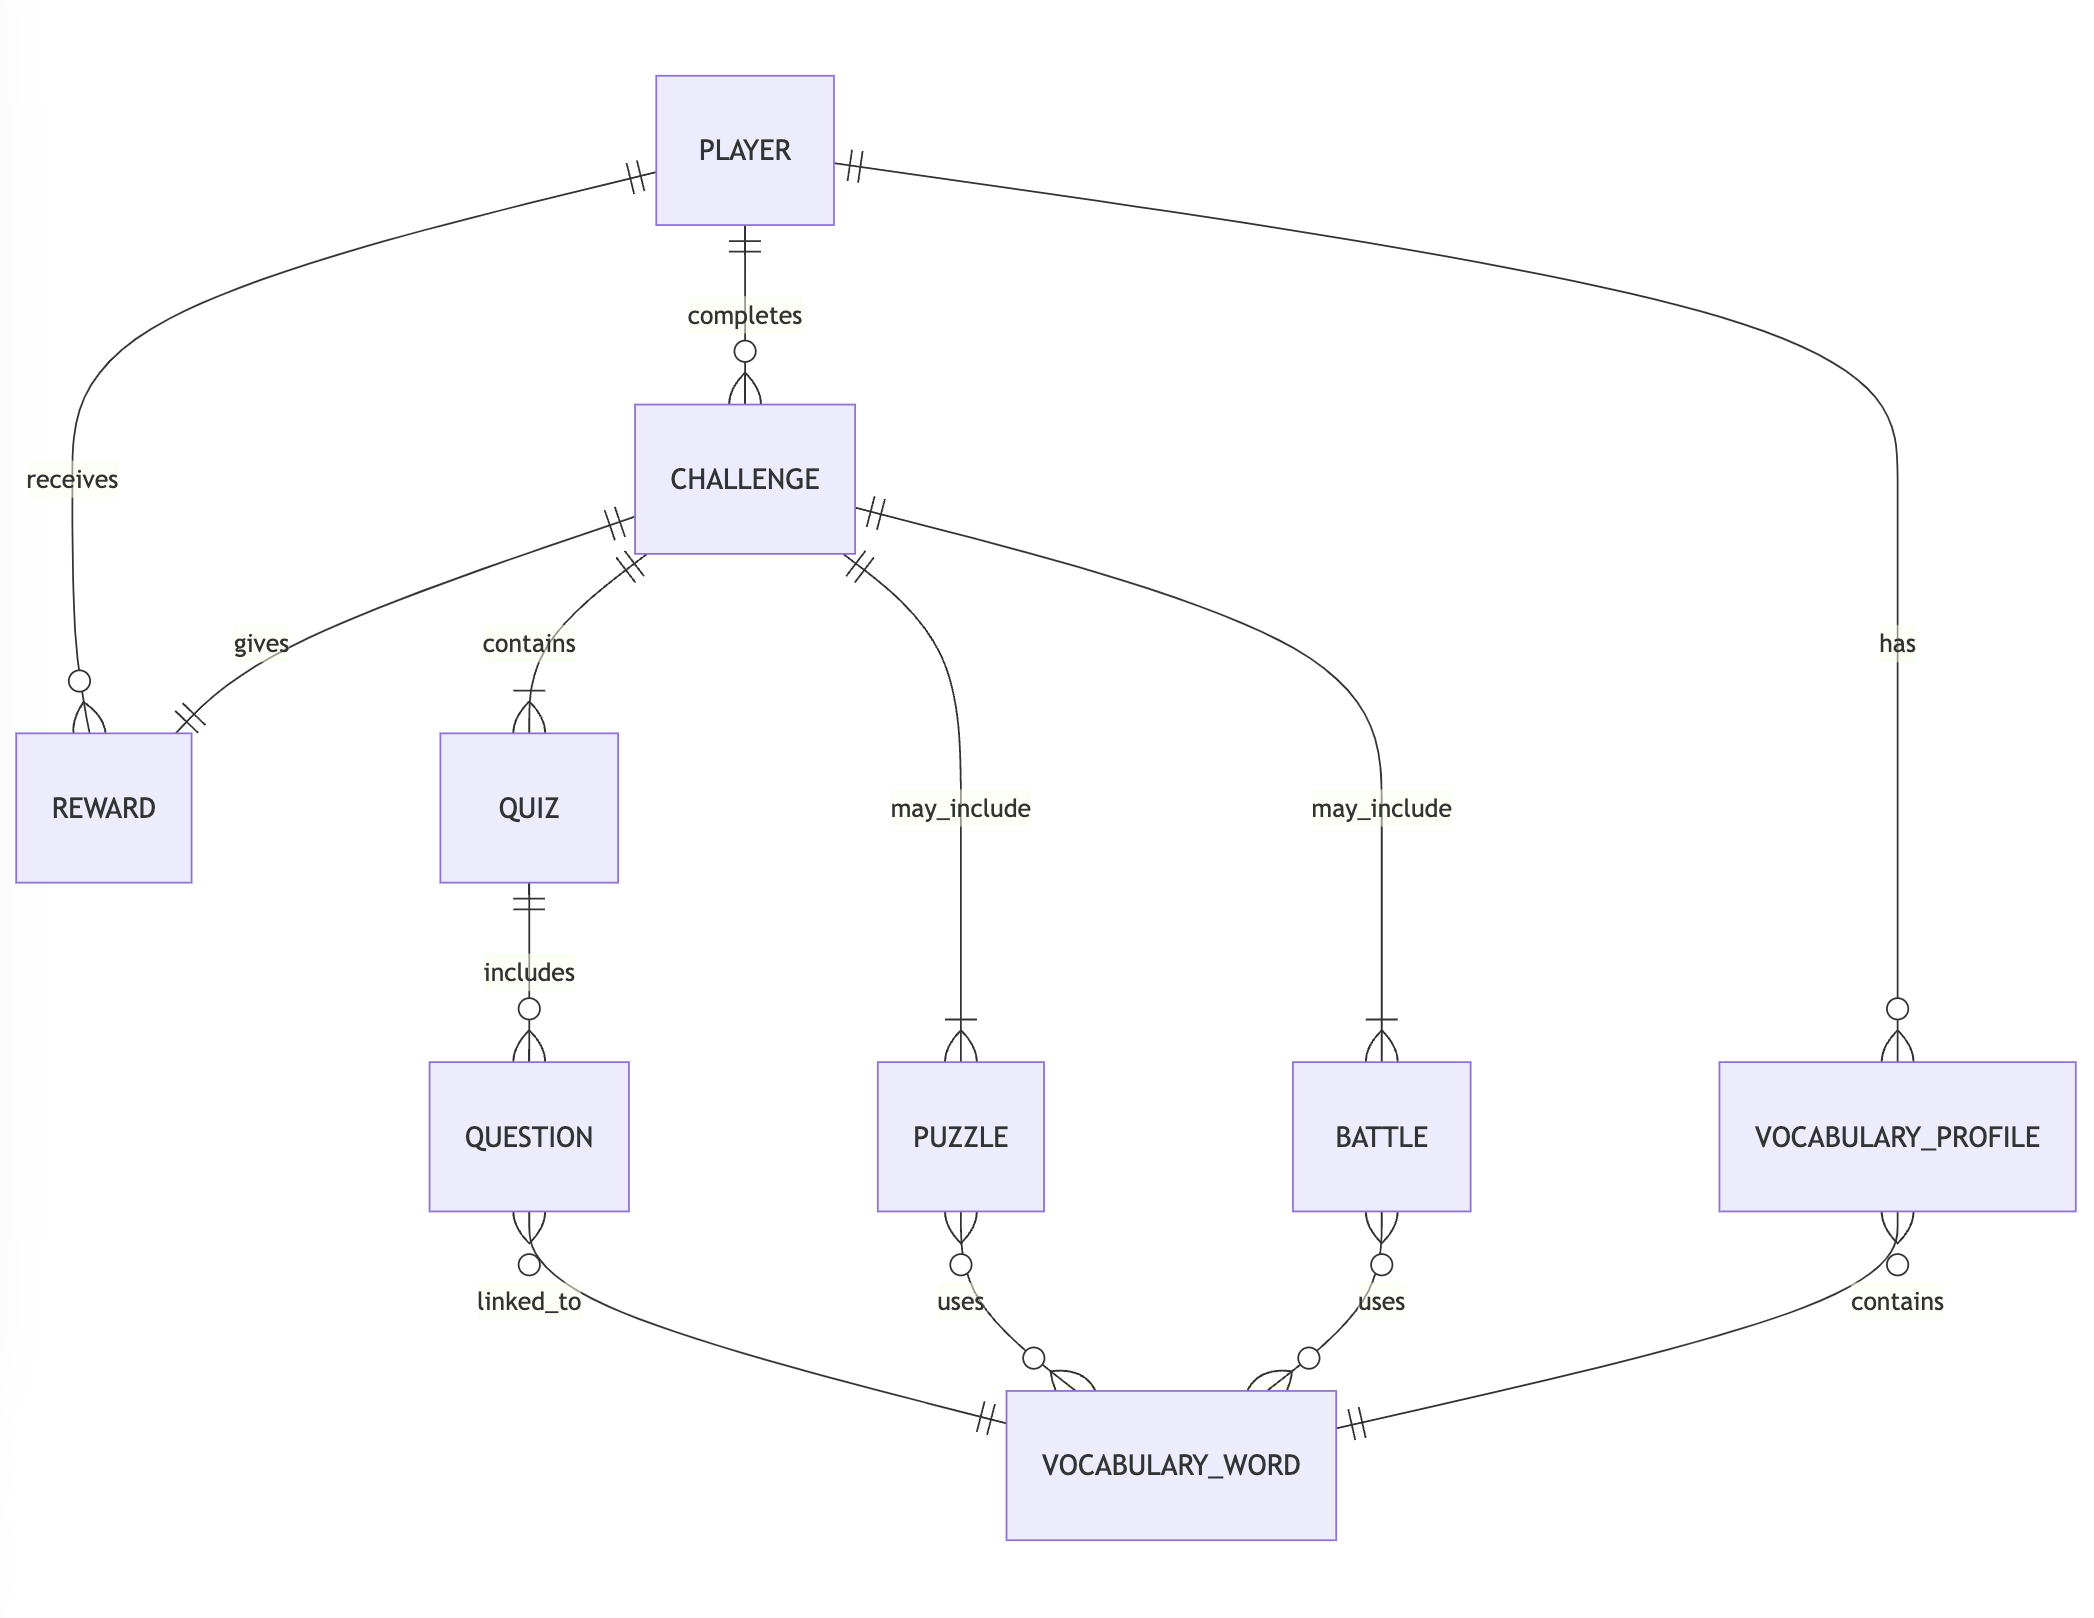
\includegraphics[width=0.85\textwidth]{assets/ku/er_diagram.png}
    \caption{Domain Model of Spell Splash}
    \label{fig:domain-model}
\end{figure}

\section{Design Class Diagram}
\label{section:design-class-diagram}
<TIP: Showcase a design class diagram for your project and explain
how it works here. You can group classes into packages or layers to communicate your
design better./>

\section{Sequence Diagram}
\label{section:sequence-diagram}
<TIP: Sequence diagrams describe how the software runs at runtime.
You do not have to create a sequence diagram for every scenario. However,
there should be one for all the main ones./>

<ChatGPT: Creating a sequence diagram for every use case is not
strictly necessary, but it can be a valuable tool in certain situations. Sequence
diagrams are particularly useful for illustrating the interactions between different
components or objects in a system over time, showcasing the flow of messages
or actions between them./>

\section{Algorithm}
\label{section:algorithm}
<TIP: Optional, If you are working on a research project that proposes a new
algorithm, you can describe your algorithm here. It can be in the form of
pseudocode or any diagram that you deem appropriate./>